
\documentclass[12pt,a4paper]{article}

\usepackage[utf8]{inputenc}
\usepackage{amsmath, amssymb, amsthm}
\usepackage{geometry}
\usepackage{tikz}
\usetikzlibrary{shapes.geometric, arrows}

\geometry{margin=2cm}

% Estilos TikZ
\tikzstyle{startstop} = [rectangle, rounded corners, minimum width=3cm, minimum height=1cm,text centered, draw=black, fill=red!30]
\tikzstyle{process} = [rectangle, minimum width=3cm, minimum height=1cm, text centered, draw=black, fill=blue!20]
\tikzstyle{decision} = [diamond, minimum width=3cm, minimum height=1cm, text centered, draw=black, fill=green!20]
\tikzstyle{data} = [parallelogram, minimum width=3cm, minimum height=1cm, text centered, draw=black, fill=yellow!20]
\tikzstyle{arrow} = [thick,->,>=stealth]

\title{Formalização Matemática e Fluxograma do Pipeline de Geração de Vídeo}
\author{}
\date{}

\begin{document}

\maketitle

\section{Definições e Notação}

Sejam:
\begin{align}
p &\in \mathcal{P} & &\text{Prompt textual do usuário},\\
n &\in \mathbb{Z}_{\ge 2} & &\text{Número de keyframes},\\
I_0 & & &\text{Imagem inicial de referência},\\
f &\in \mathbb{R}_{>0} & &\text{Duração do vídeo em segundos},\\
r &\in \mathbb{Z}_{>0} & &\text{Frames por segundo},\\
F_{\mathrm{frag}} &\in \mathbb{Z}_{>0} & &\text{Duração de cada fragmento (frames)},\\
F_{\mathrm{eco}} &\in \mathbb{Z}_{\ge 0} & &\text{Frames de eco},\\
s &\in (0,1] & &\text{Força de condicionamento}.
\end{align}

\section{Frames Totais e Alinhamento LTX}

\begin{equation}
F_{\mathrm{total}} = f \cdot r
\end{equation}

\begin{equation}
\operatorname{align8}(F) = 8 \cdot \operatorname{round}\!\left(\frac{F-1}{8}\right) + 1
\end{equation}

\begin{equation}
F_{\mathrm{ltx}} = \operatorname{align8}\left(F_{\mathrm{total}}\right)
\end{equation}

\section{Operadores Fundamentais}

\begin{align}
\mathcal{R} &: (I, m) \mapsto I' &&\text{Processa imagem para resolução $m \times m$},\\
\mathcal{G} &: (p, n, \mathrm{meta}(I_0)) \mapsto [s_1,\dots,s_n] &&\text{Gera storyboard textual},\\
\mathcal{D} &: (I_{\mathrm{ref}}, s_{\mathrm{target}}) \mapsto q &&\text{Gera prompt de transição},\\
\Phi_D &: (q, \mathcal{C}, w, h, \mathrm{params}) \mapsto I_{\mathrm{out}} &&\text{Gera imagem condicional},\\
\Phi_L &: (q_{\mathrm{motion}}, \mathcal{C}, w, h, \mathrm{params}) \mapsto (V, N) &&\text{Gera fragmento de vídeo},\\
T_{\mathrm{keep}} &: (V, k) \mapsto V' &&\text{Mantém primeiros $k$ frames de $V$},\\
E_{-n} &: (V, n) \mapsto V_{\mathrm{eco}} &&\text{Últimos $n$ frames de $V$},\\
C &: [V_1,\dots,V_m] \mapsto V_{\mathrm{final}} &&\text{Concatenação de clipes}.
\end{align}

\section{Função Total}

\begin{align}
\mathcal{F}(p,n,I_0,f,r,F_{\mathrm{frag}},F_{\mathrm{eco}},s,\mathrm{params}) &= V_{\mathrm{final}},\\
\mathbf{K} &= \operatorname{Keyframes}(p,n,I_0),\\
\mathcal{V} &= \operatorname{Fragments}(\mathbf{K}, p, F_{\mathrm{ltx}}, F_{\mathrm{frag}}, F_{\mathrm{eco}}, s),\\
V_{\mathrm{final}} &= C(\operatorname{PostTrim}(\mathcal{V})).
\end{align}

\section{Fluxograma do Pipeline}

\begin{center}
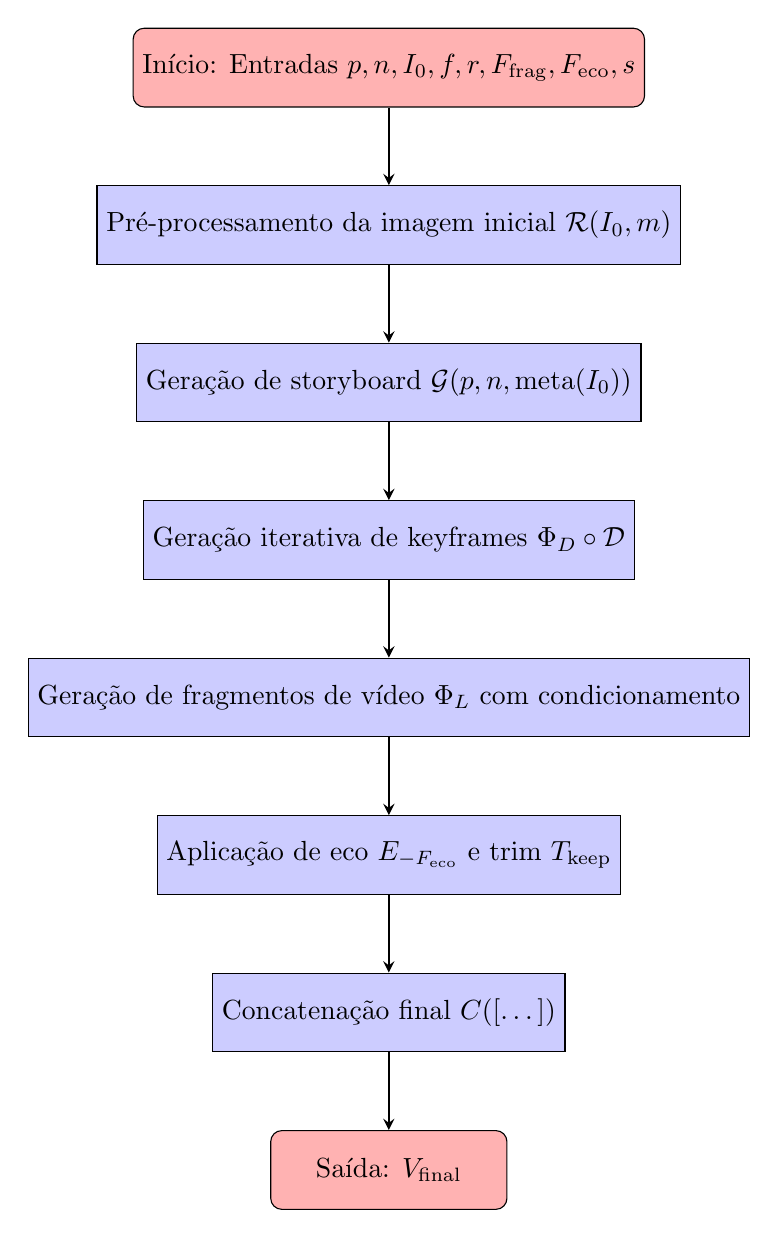
\begin{tikzpicture}[node distance=2cm]
\node (start) [startstop] {Início: Entradas $p, n, I_0, f, r, F_{\mathrm{frag}}, F_{\mathrm{eco}}, s$};
\node (pre) [process, below of=start] {Pré-processamento da imagem inicial $\mathcal{R}(I_0, m)$};
\node (story) [process, below of=pre] {Geração de storyboard $\mathcal{G}(p, n, \mathrm{meta}(I_0))$};
\node (keys) [process, below of=story] {Geração iterativa de keyframes $\Phi_D \circ \mathcal{D}$};
\node (frag) [process, below of=keys] {Geração de fragmentos de vídeo $\Phi_L$ com condicionamento};
\node (eco) [process, below of=frag] {Aplicação de eco $E_{-F_{\mathrm{eco}}}$ e trim $T_{\mathrm{keep}}$};
\node (concat) [process, below of=eco] {Concatenação final $C([\dots])$};
\node (end) [startstop, below of=concat] {Saída: $V_{\mathrm{final}}$};

\draw [arrow] (start) -- (pre);
\draw [arrow] (pre) -- (story);
\draw [arrow] (story) -- (keys);
\draw [arrow] (keys) -- (frag);
\draw [arrow] (frag) -- (eco);
\draw [arrow] (eco) -- (concat);
\draw [arrow] (concat) -- (end);
\end{tikzpicture}
\end{center}

\section{Precondições / Erros}

A função $\mathcal{F}$ é indefinida se:
\begin{enumerate}
    \item $I_0$ ausente ou inválida.
    \item $n < 2$.
    \item $F_{\mathrm{frag}} > F_{\mathrm{total}}$.
    \item Falha em $\Phi_D$ ou $\Phi_L$.
    \item Parâmetros essenciais ausentes (ex.: chaves de API).
\end{enumerate}

\end{document}
